\chapter{Experimental Procedures}

\section{(6,5) Carbon Nanotube Sample Properties}

\subsection{Sample Preparation}
The sample preparation procedure is well described by Ref \cite{ichinose2017extraction}. For preparing a high-purity (6,5) sample, the process starts with obtaining a CoMoCat solution (Sigma-Aldrich) containing several different chiralities. Gel chromatography is then performed on this mixture to isolate a solution containing a high concentration of (6,5) nanotubes. Adding sodium deoxycholate (DOC) as surfactant to prevent nanotubes from clumping together to form bundles. About 4 percent of solution is DOC. Sample is contained in a quartz cuvette with an optical path length of 1 mm.

%Include figure of absorption spectrum
\subsection{Sample Absorbance Spectrum}

Here, absorbance is defined as 
\begin{equation}
A = \log_{10}(-T),
\end{equation}
where $T$ represents the transmission through the sample. 
This is absorbance spectrum of sample. We can see E11, phonon sideband, and E22 within this spectral window. Other peaks in the sample emerge from exciton resonances of (9,1) and (6,4) nanotubes.

\begin{figure}[H]
	\centering
	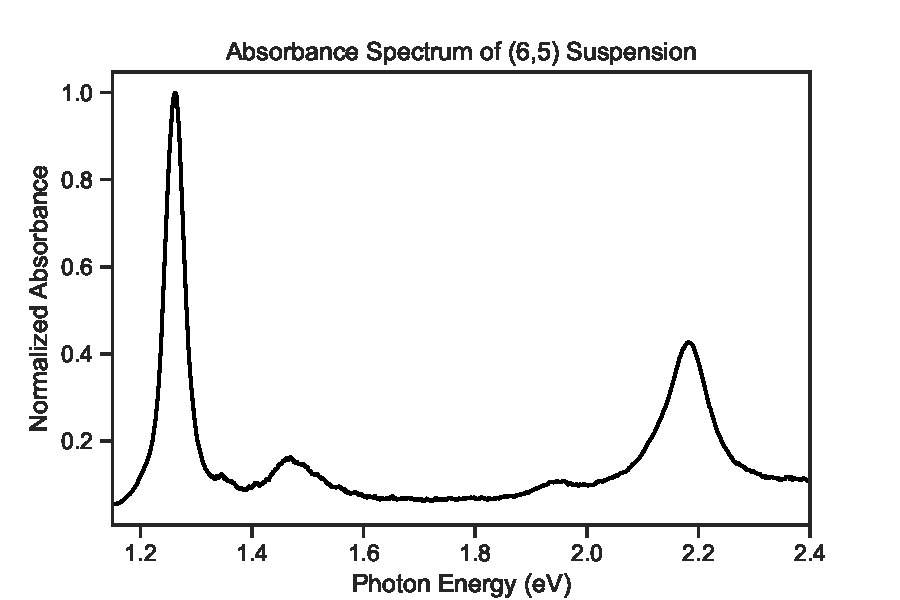
\includegraphics[scale=0.7]{images/chapter_methods/sample_absorbance}
	\caption{ Absorbance spectrum of (6,5) sample.}
	\label{fig:sample_absorbance}
\end{figure}

\section{Experimental Apparatus for Pump-Probe Spectroscopy}

%include figure of setup
\subsection{Overview}
{\color{red} Add a brief summary describing pump-probe spectroscopy and how that is done in this apparatus}.
A motorized stage in the path of optical pump beam is used to alter the optical path length of pump beam. 
Setup is equipped with an optical shutter placed in the optical path traveled by the pump beam. At each time delay, measure transmission of the probe beam with the pump beam blocked and with the pump beam unblocked by the shutter.  

Pump and probe beams are focused onto surface of the sample. This is a non-collinear geometry, meaning that pump and probe do not propagate toward the sample in a parallel trajectory. 

\begin{figure}[h]
	\centering
	\includegraphics[scale=0.7]{example-image-a}
	\caption{ Schematic Diagram of the Experimental Apparatus}
	\label{fig:sample_absorbance}
\end{figure}


\subsection{Chirped Pulse Amplifier and Optical Parametric Amplifier}
Laser is Clark MXR-2010, 1 KHz repetition rate, 150 fs pulse duration, and central wavelength of 775 nm. Operates using chirped pulse amplifier technique. 

All of the power is delivered to the OPA. OPA generates signal and idler beams. {\color{red} Briefly describe process of generating signal and idler beams}. BBO crystal added to generate SHG of signal which is used as the resonant E22 pump excitation. Signal of OPA is used to generate white light continuum in a sapphire crystal. 

\subsection{Filters}
 Wavelength separator used to seperate SHG and fundamental signal. {\color{red} Describe what wavelength separator is and mechanism for wavelength separation}.
 
\subsection{White Light Continuum Probe}

{\color{red} Briefly describe process by which probe is generated}

\subsection{Spectrometer}
The probe is collected into an optical fibre which sends this beam to a spectrometer equipped with a charge-coupled device (CCD) camera. Camera allows to measure the intensity of several wavelengths of probe beam simultaneously. 

\subsection{Pump and Probe Spot Sizes}
Pump and probe spot sizes measured using a knife edge scan. For this, mounted a razor blade on a delay stage placed in the sample position as shown in Figure \ref{fig:beam_diameter_setup}. Measure transmitted power as a function of delay stage positioning. Average power drops as razor blade cuts into beam diameter. 

\begin{figure}[h]
	\centering
	\includegraphics[scale=0.7]{example-image-a}
	\caption{Spot Size Measurement Setup}
	\label{fig:beam_diameter_setup}
\end{figure}

Assuming that the beam diameter can be approximated as a gaussian distribution, we can compute the spot size by fitting this data with the equation 

\begin{equation}
	P = P_0 + P_{max}/2 \left( 1 - \mathrm{erf} \left( \dfrac{\sqrt{2}(x - x_0)}{w} \right) \right),
\end{equation}

which this represents the cumulative distribution of a Gaussian measured and used to obtain the beam diameter $w$. Here $P_0$ represents the baseline of the power meter observed when the beam is fully blocked, erf is the standard error function, $P_{max}$ is the maximum power of the beam, $x$ is coordinate describing lateral position of the razor blade and $x_0$ represents position of razor blade when the razor blade blocks 50\% of the total power.  



\begin{figure}[h]
	\centering
	\includegraphics[scale=0.7]{example-image-a}
	\caption{Example measurement of beam diameter for pump and probe. Solid lines are fits to the data using function defined in equation}
		\label{fig:beam_diamter_measurement}
\end{figure}



